%%% LEXICON %%%
% Block: A literal block on the workspace (like a move block)
% Chain: A series of connected blocks.
% Program: All chains on the workspace.
% Workspace: The canvas where blocks are.
% Cognative Load: The amount of thinking needed to complete a task.
% Utterance: What is said by the user
% Recognition: What the speech recognition "hears" from the user
% Correction: The outcome of our correction algorithm on the recogition
% Toolbox: Where the available blocks can be found 

\documentclass[]{article}

\usepackage{amsmath, amssymb, xspace, mathalfa, algorithm, algpseudocode, hyperref, graphicx}
\hypersetup{colorlinks=True, linkcolor=blue}
\graphicspath{ {images/} }
\usepackage{amsmath, amssymb, xspace, mathalfa}
\usepackage{algorithm}
\usepackage{algpseudocode}

\title{Voice Programming in Computer Science Education}

\begin{document}
\maketitle

\section{Introduction}

Our goal is to create a voice enabled platform that uses machine learning to allow 
anyone to learn the fundamentals of computer science. Currently, we seek to reduce the amount
of cognitive load required to be introduced to programming concepts, which would give more 
students opportunities in computer science. 
\\ 
Voice programming looks to benefit both new and experienced programmers.  
Google Blockly is a simple language that allows us to create a robust programming grammer 
that can be used of people of all ages. In addition to discovering solutions to voice 
recognized programming, our project will help teach people who are unable to use a traditional mouse and keyboard.

\subsection{What are the results or outcome of the project?}

\section{HCI Principles}

\subsection{What HCI principles were kept in mind in the design of our system?}

\subsection{How did those HCI principles influence our design decisions?}

\section{Blockly}

\subsection{What is the Blockly environment?}
Google Blockly is a JavaScript library that creates a visual block programming 
enviornment where core computer science logic can be taugh, such as conditionals and 
looping. Blockly is run in the web browser, which gives the opportunity for mobile development. We chose Google Blockly over other block based languages due to its easy to
work with and customizable API.

\subsection{How are blocks arranged horizontally? What language do we use to describe this?}

\subsection{How are blocks arranged vertically? What language do we use to describe this?}

In Blockly, there is the ability to allow several chains of blocks to be run while
in the workspace. The order of execution causes the topmost chain of blocks (topmost 
being indicated by the top block in the chain's y location). Normally, users interact
with Blockly through looking at the workspace and adding blocks to the workspace by
using the toolbox. In order to move blocks from the toolbox to the workspace, users
must click and drag using a mouse. 
\\\\ \textbf{Available blocks}
\begin{itemize}
\item $\textbf{move}$: moves the tutle forward
\item $\textbf{turn}$: turns the turtle, can decide between left or right turning and angle of turning  1,45,72,90,120,140 degrees
\item $\textbf{repeat}$: repeats the blocks found inside, can decide to repeat either 2,3,4,5 or 360 times
\item $\textbf{pen}$: can decide between up/down, up stops the turtle from drawing a line, down makes the turtle's movements draw lines again
\end{itemize}
Users must refer to blocks as the block number that is shown on the block\\
\textbf{Users can move blocks in 2 ways}:
\begin{itemize}
\item \textbf{Connect block $<$ID$>$ under block $<$ID$>$}: allows user to move blocks and chains of block under any block or chain of blocks
\item \textbf{Connect block $<$ID$>$ inside block $<$ID$>$}: allows user to move block and chains of blocks inside of a repeat block
\end{itemize}
\textbf{delete block $<$ID$>$}: deletes a block,  unless the block is the head of a chain of blocks, then this command deletes the entire chain of blocks. 
\subsubsection{How does separating blocks work?}


\section{Turtle}

\subsection{What is the turtle game?}

\subsection{What set of blocks are available to complete the game?}

\subsection{What do these blocks do?}

\subsection{Why is the game divided into levels?}

\subsection{How do the levels serve to teach different programming concepts?}


\section{Speech}

\subsection{Why did we decide to model speech using a} % This subsection heading might be incomplete?

\subsection{What choices did we make as we designed that grammar?}

\subsection{What commands are available in that grammar?}

\subsection{How do the user interface commands described earlier map to the commands in the grammar?  }

\section{Speech recognition}

\subsection{How do we perform the speech recognition? What do we use?}

\subsection{What tradeoffs are there in our decision by comparison to alternatives? What was gained and what lost?}

\clearpage

\section{Suggestions}

\subsection{Why do we give suggestions to the user? What HCI principle is behind this?}

%\subsection{What is basis on which a speech suggestion is made? What circumstances trigger it?}
%\subsection{What are the limitations of the current method and what future work might improve upon it?}
%\subsection{Show an example of the suggestions box and workspace before and after an operation}
We modify the suggestions list when we believe it could be useful for the user. For example, when there is a repeat block on the canvas, we suggest that the user connects a block inside of the repeat block, to make use of the repeat block. However, our current suggestions system is quite limited. It provides generic suggestions, not specific to the block IDs. For example, when an empty repeat block is on the canvas, we suggest that the user ``Connect block 2 inside block 1'' with these exact block IDs, regardless of what the block ID of the repeat block is. Finally, we provide an example in \hyperref[SuggestionsBeforeAndAfter]{Table \ref{SuggestionsBeforeAndAfter}} of the suggestions box with the corresponding workspace before and after adding the first block. \\
\begin{table}
	\caption{Example of suggestions before and after adding the first block to the workspace.}
	\label{SuggestionsBeforeAndAfter}
	\begin{tabular}{cccc}
		\hline
		when & workspace & suggestions \\\hline
		\\
		before & 
\includegraphics{suggestions_before_workspace.jpg} & 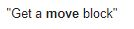
\includegraphics{suggestions_before.jpg} \\\hline
		\\
		after & 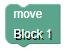
\includegraphics{suggestions_after_workspace.jpg} & 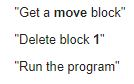
\includegraphics{suggestions_after.jpg} \\\hline
	\end{tabular}
\end{table}

\subsection{What is basis on which a speech suggestion is made? What circumstances trigger it?}

\subsection{What are the limitations of the current method and what future work might improve upon it?}

\subsection{Show an example of the suggestions box and workspace before and after an operation}

\section{Corrections}
\textit{Utterance:} A single command given by the programmer\\
\textit{Recognition:} What the speech reognition software recogizes an utterance as\\
\textit{Correction:} The proposed utterance given a recognition, calculated using correction algorithm\\

%\subsection{Give an example of a common recognition error that falls out of the grammar}
%\subsection{What algorithm was used to correct recognition?}
%\subsection{If there are any parameters to be fit in this correction algorithm, how were they fit?}
As previously described, we use the webkitspeechrecognition speech API to capture user commands. However, the API has a hard time understanding commands from our grammar. We hypothesize that the API expects ordinary English, and as a result, phrases like ``get a turn block'' or ``change 4 in block 3 to 5'' are often recognized incorrectly by webkitspeechcrecognition. We developed a \hyperref[CorrectionAlgorithm]{novel algorithm} to correct incorrectly recognized phrases (``recognitions'') to what we hope are the intended commands (``utterances''). The algorithm finds the command with minimal phoneme edit distance from the set of possible commands for a given workspace.
\begin{algorithm}
	\caption{Correction Algorithm}\label{CorrectionAlgorithm}
	\begin{algorithmic}[1]
		\Procedure{Correct}{recognition, workspace}
		\State $recognitionPhoneme \leftarrow stringToPhoneme(recognition)$
		\State $allPossibleCommands\leftarrow generateAllPossibleCommands(workspace) $
		\State $minimumEditDistance \leftarrow \infty$
		\State $minimumEditDistanceCommand = recognition$
		\For{$command$ in $allPossibleCommands$}
			\State $commandPhoneme \leftarrow stringToPhoneme(command)$
			\State $editDistance \leftarrow findMinimumEditDistance(recognitionPhoneme, commandPhoneme)$
			\If{$editDistance < minimumEditDistance$}
				\State $minimumEditDistanceCommand = command$
				\State $minimumEditDistance = editDistance$
			\EndIf
		\EndFor
		\State \Return{$minimumEditDistanceCommand$}
		\EndProcedure
	\end{algorithmic}
\end{algorithm}\\
Furthermore, if the minimum edit-distance command is too far from the original recognition, we reject the correction and simply notify the user that we didn't understand their command. Our notion of ``too far'' is more concretely defined by a maximum modification factor which defines the the number of phoneme edits that can be made as a percentage of the number of phonemes in the recognition. As such, there is no fixed maximum number of edits, as this could give different performance for different string lengths. We determined the threshold in the following way.
\subsection{If there are any parameters to be fit in this correction algorithm, how were they fit?}
\subsubsection{What statistical procedure was use?}
\subsubsection{What data was gathered?}
\subsubsection{What assumptions were made that could be considered weaknesses of the model?}
\subsection{Give an example of a common case that the corrections algorithm, as currently implemented, fails on}

\section{Layout}

%\subsection{How are commands interpreted visually?}
%\subsection{Where do new blocks go?}
%\subsection{How are blocks reordered when one is moved?}
%\subsection{What happens if the user runs out of space on the workspace?}
%\subsection{Describe the layout algorithm in pseudocode}
%\subsection{Show an example of the a before and after with the layout algorithm}
%\subsection{Are there any cases that currently give problems for the layout algorithm?}

As the user writes a program, certain locations on the workspace fill with blocks.
This presents a challenge: what should happen when blocks overlap with one another?
For our system to be practically useful, it must avoid introducing such visual impairments,
which may prevent the user from issuing commands (e.g. if they cannot see a block ID)
or which may introduce unnecessary cognitive load.

Blockly by default places new blocks at the top left of the workspace, even if the new block
will overlap an old block. Similarly, when Blockly connects one block to another, the resulting chain
might overlap another chain.

We devise simple layout algorithms for each case. To make this formal, we view
the workspace as a 2D plane.

% TODO(evanfredhernandez): Diagrams for these algorithms. And pseudocode?

\textbf{Adding Blocks} (1) Find the vertically lowest block on the workspace.
Let $y$ be the vertical coordinate of its lower left corner. (2) Place the new block
such that its top left corner is at $(20, y)$, that is, below the lowest block on the
workspace, 20 pixels right of the flyout.

\textbf{Moving Blocks} Suppose the user has just connected one block to another, and the
resulting chain now overlaps $n$ blocks. We repair the layout by moving the $n$ conflicting
blocks via the procedure below. For brevity, let $W$ and $H$ be the width and height of
the entire workspace, respectively, let $b$ be the block to be moved, and let
$w_b$ and $h_b$ be the width and height of $b$ and its children. Additionally define $m$
to be a small margin.
\begin{enumerate}
\item{Construct the set of candidate new locations: $$C = \{(x, y) = (rm, sm) : r, s \in \mathbb{Z}, x \le W, y \le H\}$$}
\item{For every $(x,y) \in C$ check if there is no block within the box bounded by the four points:
	$$(x,y), (x + w_b, y), (x, y + h_b), (x + w_b, y + h_b)$$
Let $(\hat{x}, \hat{y})$ be the first found satisfying that condition. If none is found, set $\hat{x} = \hat{y} = m$.
}
\item{Move $b$ so that its top left corner is located at $(\hat x, \hat y)$.}
\end{enumerate}
We choose $m = 20$ (pixels) because it is small enough to preserve space on the workspace,
and large enough to prevent Blockly from automatically connecting nearby blocks.

\section{Related Work}

\subsection{What is the related work in speech interfaces for programming?}

\subsection{What is the related work in speech interfaces for computer science education?}


\section{Future Work}

\end{document}
